\problemname{Fredrik's Pizzeria}
\noindent

Your friend Elsa works as a night guard at Fredrik's pizzeria.
The pizzeria has $N$ rooms and $M$ undirected corridors, numbered from $1$ to $N$ and $1$ to $M$ respectively.
She is currently in room $1$.
The night shift just ended, and she wants to go home through the exit in room $2$.
Unfortunately, there is a malicious rat in room $3$ that is trying to stop her.
To protect herself, each corridor has an electronic door that she can close.
Neither Elsa nor the rat can pass through a closed door.
She can open and close doors however she wants, with one requirement:
each door is linked to \textbf{exactly} one other door.
If two doors are linked, it means that if one is closed, the other must also be closed.
Likewise, if one is open, the other must also be open.
Doors being linked with each other is symmetric, which means that if door $a$ is linked to door $b$, then door $b$ is linked to door $a$.

Since the control panel is in her office in room $1$, she must decide which corridors to open or close before leaving the office.
Once she has left the office, her only chance is to have closed doors so that the rat cannot reach her through corridors with open doors, while she can reach the exit through corridors with open doors.
Even if her office were right next to the exit, the rat is so fast that she would not be able to get out in time if the rat could reach her.

Determine whether there is a way to close doors so that Elsa can get out, while the rat
cannot reach her.

Due to fire safety regulations, it is also guaranteed that each corridor is part of at most one cycle\footnote{The definition of a cycle with $k$ ($k \geq 3$) rooms is a sequence of rooms $c_1, c_2, \dots, c_k$, where all $c_i$ are pairwise distinct and there is a corridor between $c_i$ and $c_{i+1}$. Note that there must also be a corridor between $c_k$ and $c_1$. In particular, a single room, or a pair of rooms connected by a corridor is not a cycle, since $k < 3$ in those cases.}.

\section*{Input}
The first line of input contains the integers $N$ and $M$ ($3 \leq N \leq 2 \cdot 10^5$, $2 \leq M \leq 2 \cdot 10^5$),
the number of rooms and corridors in the pizzeria. It is guaranteed that $M$ is even.

The $i$th of the following $M$ lines each contains the integers $u$, $v$ and $l$ ($1 \leq u,v \leq N$, $u \neq v$, $1 \leq l \leq M$, $l \neq i$),
meaning that there is a corridor between rooms $u$ and $v$, and that this corridor is linked with corridor number $l$.
The corridors are given in the same order as they are numbered.
It is guaranteed that there is at most one corridor between each pair of rooms.
It is also guaranteed that a corridor is linked with a \textit{different} corridor and that the linking of corridors is symmetric: corridor $l$ is linked with corridor $i$.

It is also guaranteed that all rooms can be reached from room $1$ if all doors are open, and that each corridor is part of at most one cycle.

\section*{Output}
Print ``\texttt{Ja}'' if it is possible to close doors so that Elsa can get out while the rat cannot reach her, otherwise ``\texttt{Nej}''.

\section*{Scoring}
Your solution will be tested on a set of test groups.
To earn points for a group, you must pass all test cases in that group.

\noindent
\begin{tabular}{| l | l | p{12cm} |}
  \hline
  \textbf{Group} & \textbf{Points} & \textbf{Constraints} \\ \hline
  $1$    & $5$        & $N, M \leq 100$ and there are no cycles. \\ \hline
  $2$    & $10$       & There are no cycles. \\ \hline
  $3$    & $12$       & $N, M \leq 100$ \\ \hline
  $4$    & $8$        & $N, M \leq 2000$ and each room is part of at most one cycle. \\ \hline
  $5$    & $15$       & $N, M \leq 2000$ \\ \hline
  $6$    & $19$       & Each room is part of at most one cycle. \\ \hline
  $7$    & $31$       & No additional constraints. \\ \hline
\end{tabular}

\section*{Explanation of Samples}
All samples will be visualized as follows:
room $1$ (the starting room) will be marked green,
room $2$ (the exit) blue,
and room $3$ (the rat's room) red.
The corridors will be colored so that corridors with the same color are linked.

In sample $1$, it is not possible because the only corridors between the exit and the rat are linked.
If Elsa chooses to open corridors $1$ and $2$, the rat will stop her.
If she closes the corridors, she will not be able to get out.

\begin{figure}[h]
  \centering
  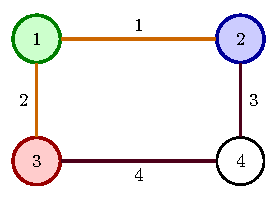
\includegraphics[width=0.4\textwidth]{sample1.pdf}
\end{figure}

In sample $2$, it is possible.
One solution is to close the pairs of doors in corridors $2,7$ and $4,5$.
Then the rat cannot reach Elsa, while she can get out by walking through rooms $1,4,6,2$.
This case could not be part of group $4$ or $6$ since room $6$ is part of
two cycles (the cycles $6,4,1,5$ and $6,7,3$).

\begin{figure}[h]
  \centering
  
\includegraphics[width=0.4\textwidth]{sample2.pdf}
\end{figure}
